\documentclass[twocolumn]{article}

\usepackage{authblk}
\usepackage{amsmath}
\usepackage{amssymb}
\usepackage{amsfonts}
\usepackage{graphicx}
\usepackage{siunitx}
\usepackage{float}

\title{\vspace{-.2in}\textbf{Modeling Random Memristive Nanowire Networks}}
\author[1,2]{Daniel Teal}
\author[3]{Dr.\ Tomonobu Nakayama}
\affil[1]{Mechanical Engineering \& Mathematics, the University of Texas at Austin}
\affil[2]{2018 iREU NNCI/NIMS Internship Program}
\affil[3]{Nano Functionality Integration Group, MANA, NIMS}
\date{}

\begin{document}

\maketitle

\section{Abstract}

Nanowires (NWs), micron-scale cylinders with high aspect ratios, are easy to precisely fabricate in many materials and dimensions. Furthermore, the junctions between crossed nanowires may form high-performance transistors, diodes, or other electronic elements. These properties make NWs appealing building blocks for future microelectronics$^1$. However, it is difficult to assemble individual NWs into circuits. Thus, we investigate the properties of easier-to-assemble random networks. Here, we study networks of polyvinylpyrrolidone (PVP)-coated Ag (Ag@PVP) nanowires. Modeling junctions as variable resistors, we describe two modes of behavior: sufficient voltage across a network causes current to rise exponentially; in its absence, the network eventually returns to its original state. Experimental measurements support this model for a time decay on the order of weeks. These networks might be used to build ephemeral memories, current switches, or planar memristors.

\section{Methods}

Although, as aforementioned, it is difficult to manufacture electronics from precisely placed individual components, bottom-up assembled networks have been used to construct structures such as reservoir computers$^2$. We investigate Ag@PVP networks in search of similarly useful emergent properties.

PVP-coated Ag NWs were formed via a wet chemistry process$^3$. NW length varied about \SI{10}{\micro\meter}, NW diameter was on the order of \SI{500}{\nano\meter}, and PVP coated the NWs in a layer single nanometers thick. Au electrodes \SI{10}{\nano\meter} thick and \SI{3}{\milli\meter} apart were sputtered on glass, on top of which were drop-cast NWs in ethanol, as shown in Figure 1, for a density near \SI{0.2}{NW\per\micro\meter^2}.

\begin{figure}[h]
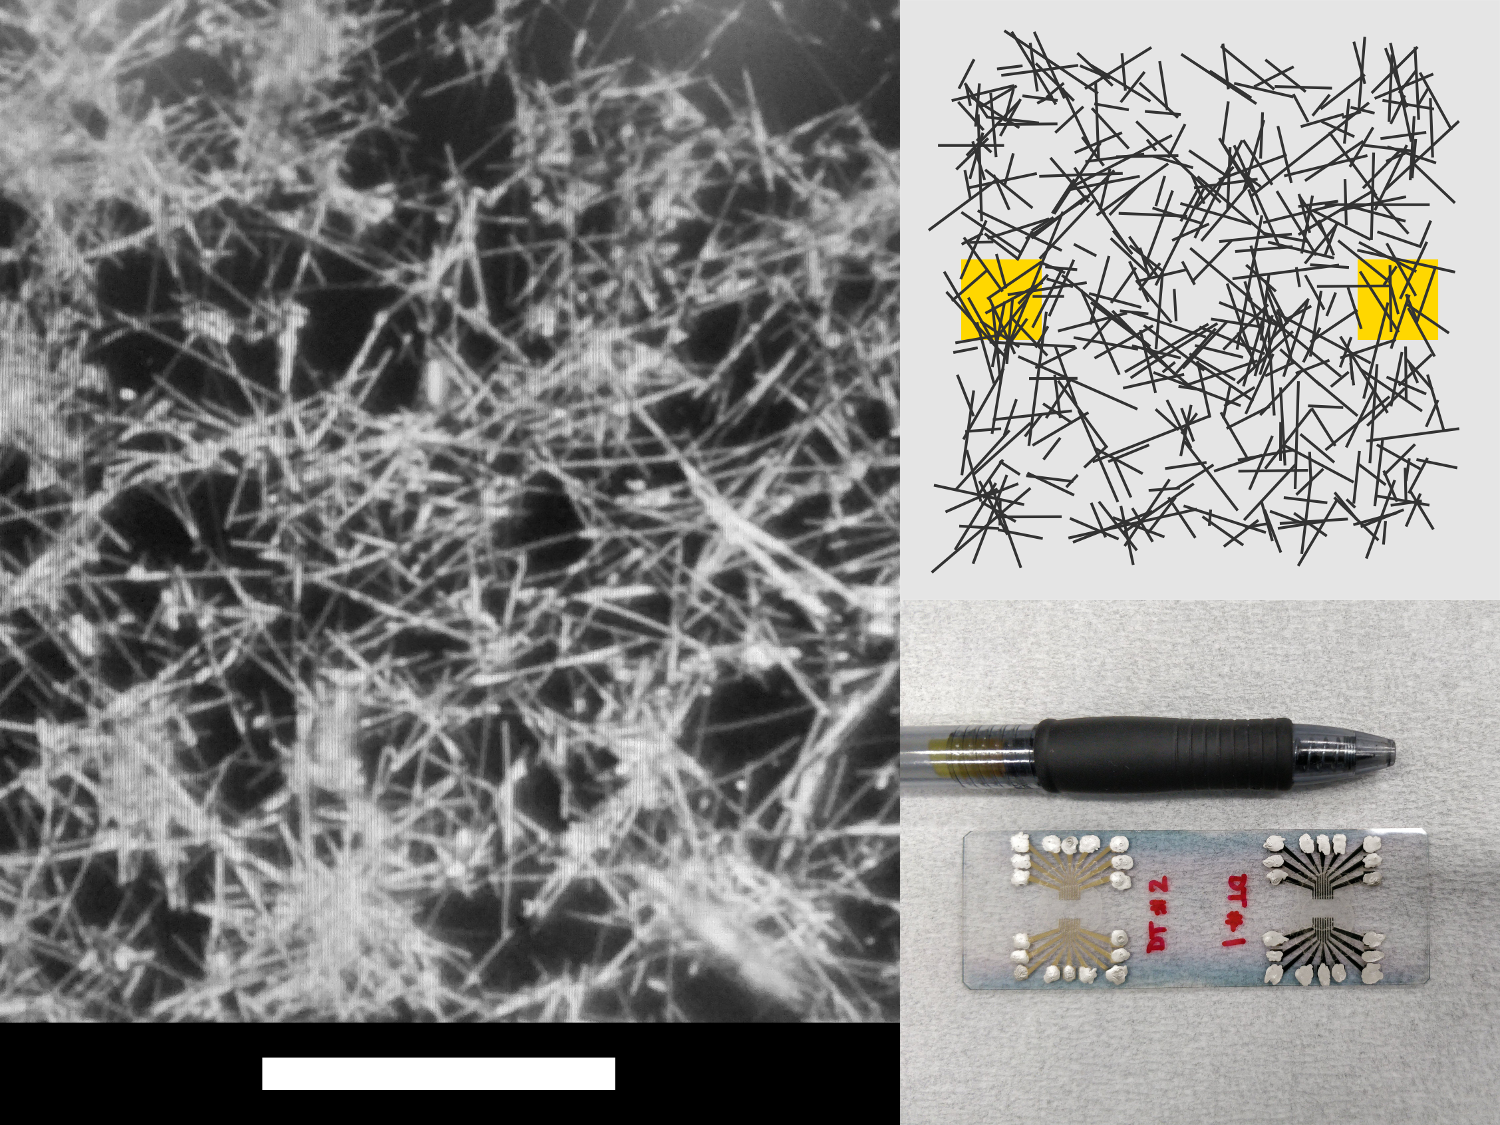
\includegraphics[width=\columnwidth]{resources/micrograph.png}
\caption{Left: micrograph of an Ag@PVP network. Scale bar is \SI{20}{\micro\meter}. Top right: visualization of a computer-simulated network with two electrodes. Bottom right: Two physical networks with gold electrodes.}
\end{figure}

\subsection{Model}

It is hard to physically measure the complete internal dynamics of the network. Instead, we construct a digital simulation that will be verified by simpler physical experiment. We model each nanowire as a line segment on a 2D plane, as shown in Figure 1, and mark any intersection between two nanowires as a junction. Electrodes are defined and connected to any overlapping nanowires. The network is treated as a resistive circuit, where a voltage is applied across electrodes, nanowires are zero-resistance wires, and junctions are presumed to be resistive connections between nanowires.

The junction model, based on the common linear memristor model and Gimzewski et al.$^2$, assumes two nanowires are separated by a thin film of PVP. Any voltage potential between the nanowires drives a small current which moves Ag ions via electromigration into the PVP film, forming a low-resistance filament. Thus the junction is an ohmic resistor with a value between low and high states with

\begin{equation} V = \left[ \frac{w}{w_{\max}} \cdot R_{on} + \left(1-\frac{w}{w_{\max}}\right) \cdot R_{off} \right] \cdot I, \end{equation}

where $w$, the width of the filament, varies between zero and $w_{\max}$, the thickness of the PVP film. In the absence of current, the filament dissolves over time. We model the change of filament width by

\begin{equation} \frac{dw}{dt} = \mu \cdot \frac{R_{on}}{w_{\max}} \cdot |I| - \frac{w}{\tau}, \end{equation}

where $\mu$ is an ion mobility constant and $\tau$ is a dissolution time constant. When the dissolution state of (2) dominates, the width decreases exponentially with half-life 

\begin{equation} ln(2)\cdot\tau, \end{equation}

and when significant current instead reinforces the formation term of (2), the junction width increases with positive second derivative and half-life

\begin{equation} \frac{R_{off}\cdot w_{\max}^2}{2\cdot\mu\cdot R_{on}\cdot V}.\end{equation}

\subsection{Simulation}

Using the model, we apply a constant voltage to two electrodes on a 250 NW network. In response, current rises asymptotically, as shown in Figure 2. Eventually, a path of low resistance is formed between the two electrodes. Filament decay may be observed indirectly in the same way by tracking the conductivity of the network under a negligible current flow.

\begin{figure}[H]
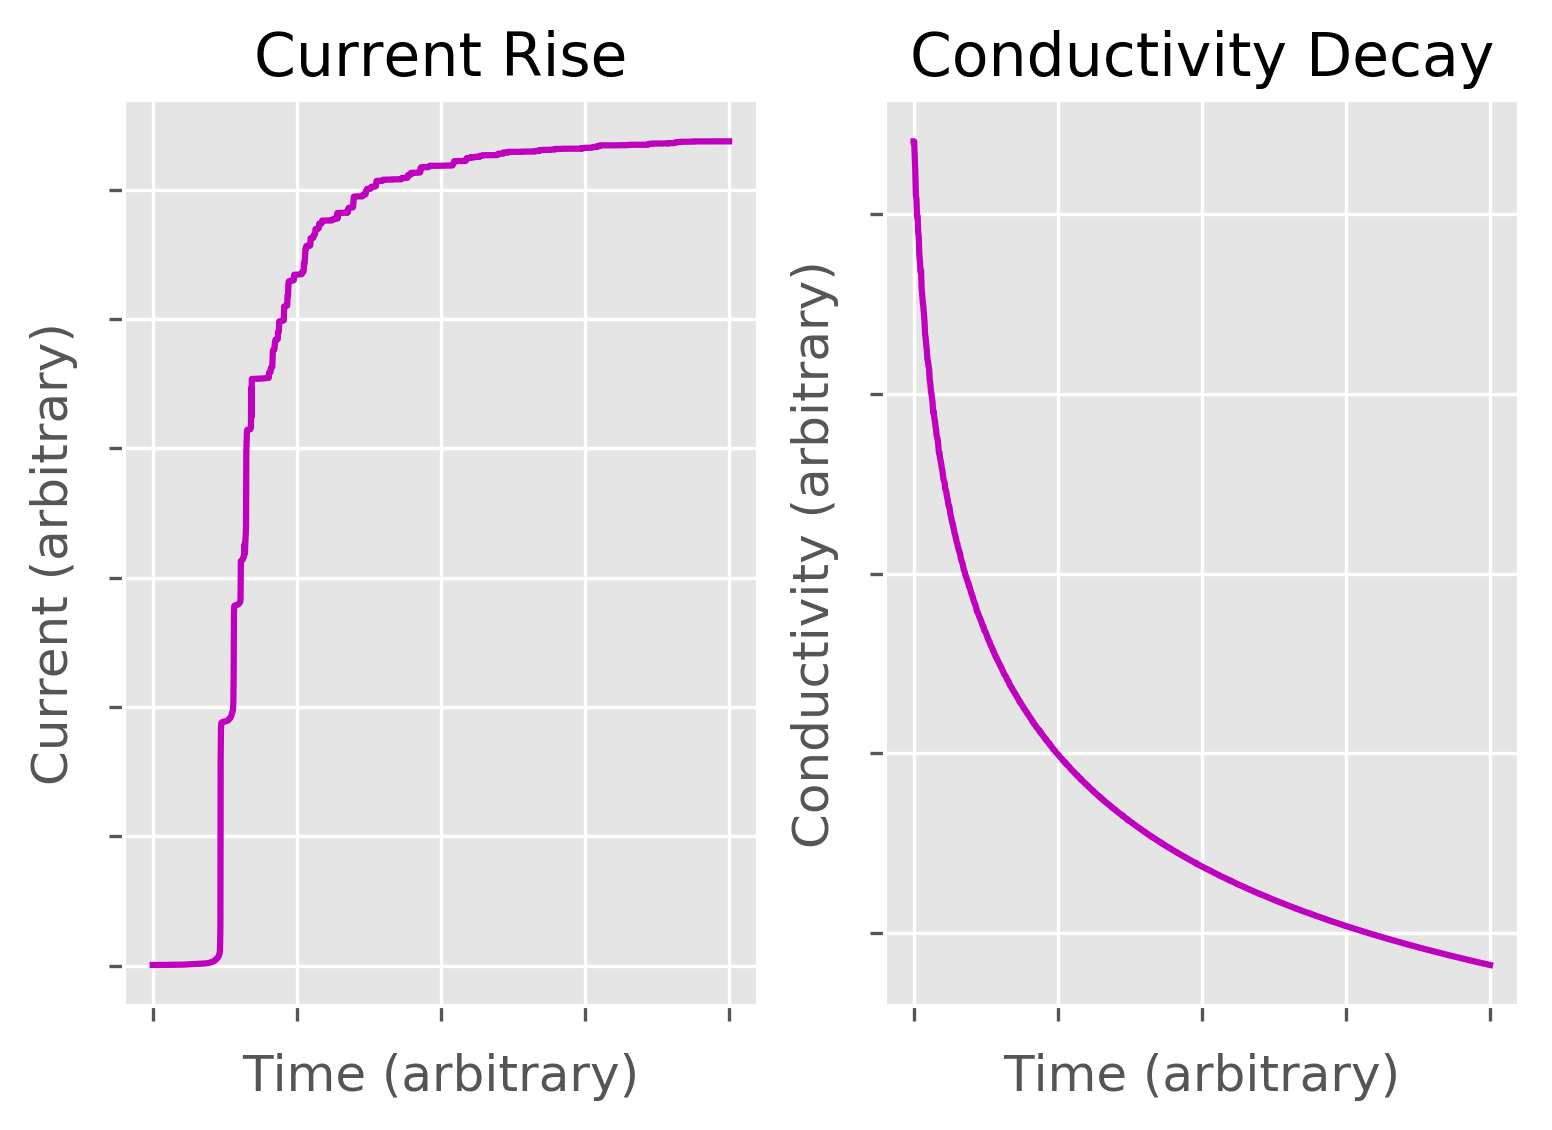
\includegraphics[width=\columnwidth]{resources/simulation.png}
\caption{Response of the simulated network to a constant voltage with arbitrary units. Left: with high voltage, current rises. Discrete steps mark individual junction filament growth. Right: with negligible voltage and current, network conductivity decreases.}
\end{figure}

\begin{figure}[H]
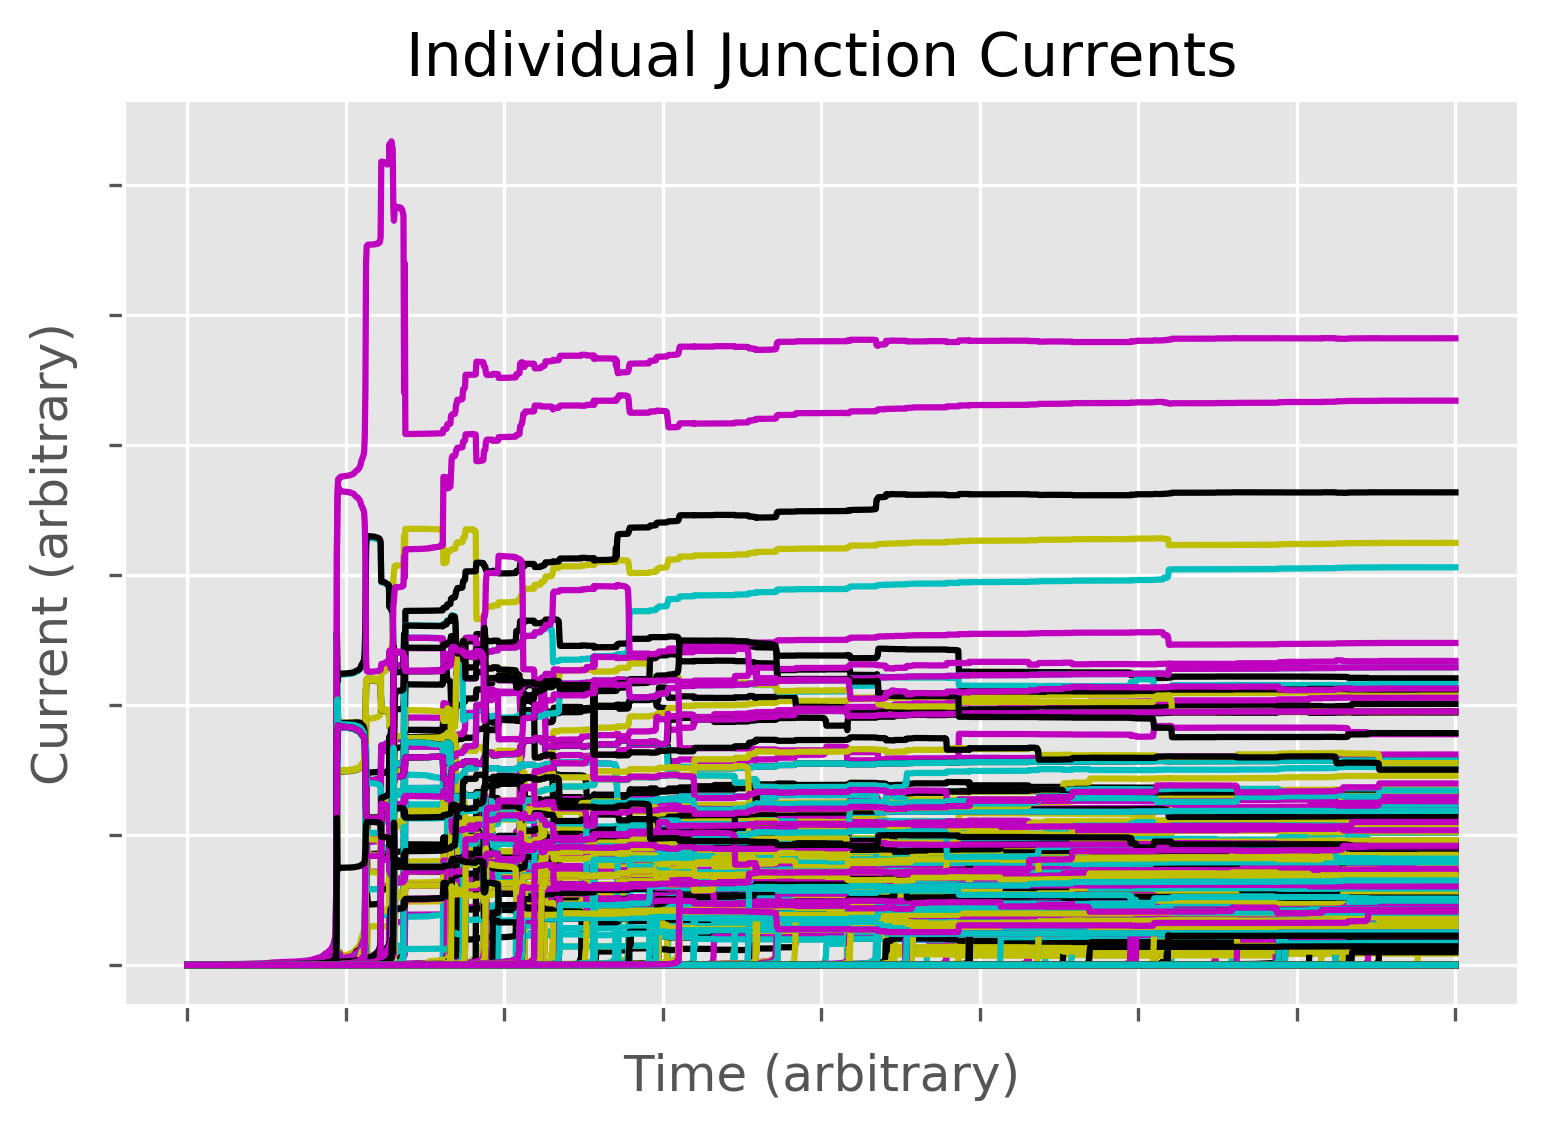
\includegraphics[width=\columnwidth]{resources/simulation_individual.png}
\caption{As current flows through the network, filament growth across a junction increases its individual flow, decreases total network resistance, and triggers a cascade of further growth.}
\end{figure}

\subsection{Experiment}

The model was supported by physical experiment. 5V applied to electrodes of multiple networks, fabricated as previously described, via a Keithley 4200-SCS system produced the current profiles of Figure 4, which mimic Figure 1. In the same way, a low 1 mV resulted in conductivity decay. Extrapolation measures the decay time constant in weeks.

\begin{figure}[h]
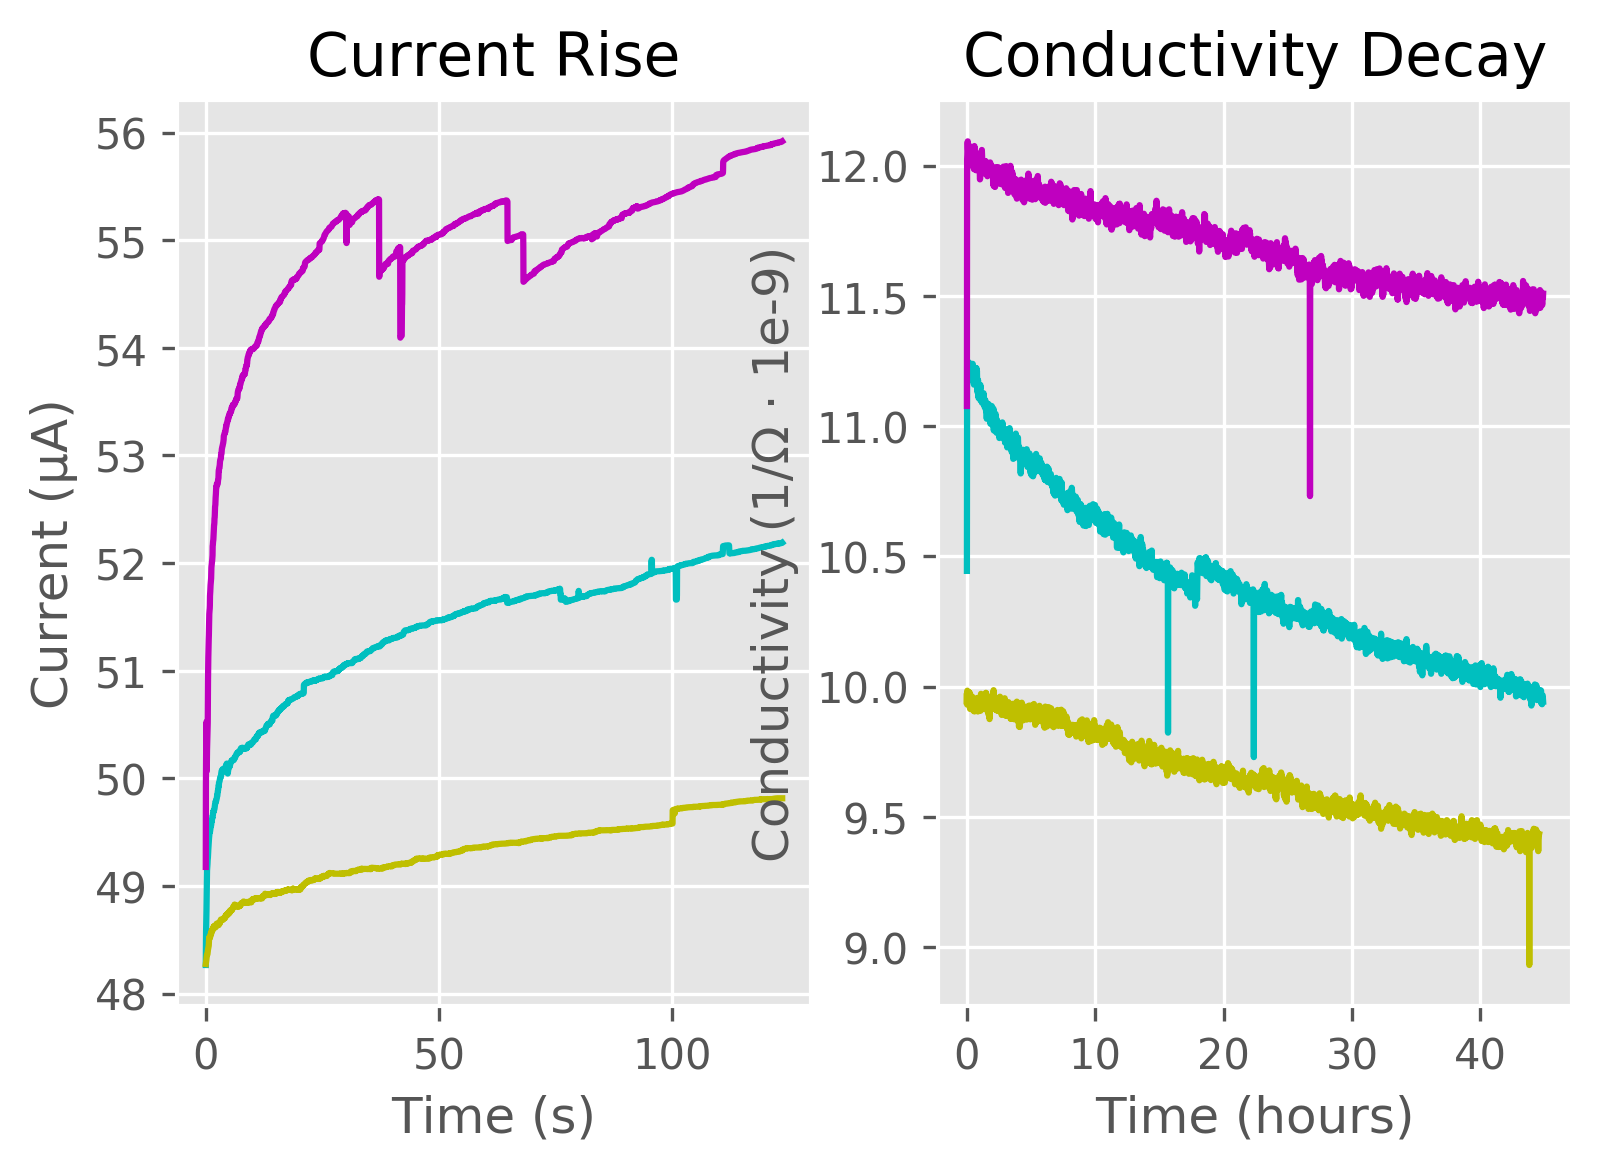
\includegraphics[width=\columnwidth]{resources/experiment.png}
\caption{Experimental responses of three Ag@PVP networks to low and high voltage, respectively, analogous to Figure 2. Left: noise is unexplained. Right: data discontinuities are due to experimental errors.}
\end{figure}

\vspace{-.15in}

\section{Conclusions \& Future Work}

Experimentally supported computer simulation of random PVP@Ag nanowire networks demonstrated two modes of behavior: an accelerating, internally chaotic rise and an exponential decay. The week-long decay constant and resistive behavior of the physical network discourages real-time reservoir computing. However, such networks could remember data via low-resistance paths for fixed amounts of time (ephemeral memory), use these paths to switch currents between multiple electrodes, or simply serve as sheet memristance. Further study of the networks should be able to improve parameter control. Addition of capacitance may improve dynamics for computational purposes.

\section{Acknowledgements}

The author thanks Dr.\ Tomonobu Nakayama and the  Nano Functionality Integration Group for hosting this project, part of the 2018 iREU internship program between NNCI and the National Institute of Materials Science (NIMS). Thanks also to organizer Dr.\ Lynn Rathbun and NSF grant OISE-1559368.

\section{References}

\begin{enumerate}

\item Lieber, C., Zhang, A., \& Zheng, G. (2016). Nanowires. New York, NY: Springer.

\item Gimzewski et al. (2013). Nanotechnology. doi:10.1088/0957-4484/24/38/384004

\item Zhang et al. (2013). Journal of Nanomaterials. doi:10.1155/2013/456098

\end{enumerate}

\end{document}